\titledquestion{Maximum area rectangle in histogram}

We are given a histogram consisting of $n$ parallel bars side by side, each of width $1$, as well as a sequence $A$ containing the heights of the bars where the height of the $i$th bar is $\mathbf{a}_i$ for $\forall \; i \in [n]$. For example, the figures below show the case where $n= 7$ and $A = \langle 6, 2, 5, 4, 4, 1, 3 \rangle$. Our goal is to find the maximum area of the rectangle placed inside the boundary of the given histogram with a \textbf{divide-and-conquer} algorithm. (Here you don't need to find which rectangle maximizes its area.)

Reminder: There do exist algorithms that solve this problem in linear time. However, you are \textbf{not allowed} to use them in this homework. Any other type of algorithms except the divide-and-conquer ones will get \textbf{no} credit.

\begin{figure}[htbp]
    \centering
    \begin{minipage}[t]{0.48\textwidth}
        \centering
        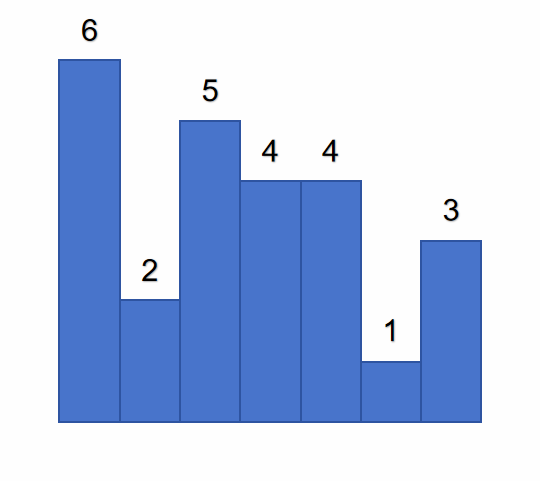
\includegraphics[width=6cm]{withnum.png}
        \caption{The Original Histogram}
    \end{minipage}
    \begin{minipage}[t]{0.48\textwidth}
        \centering
        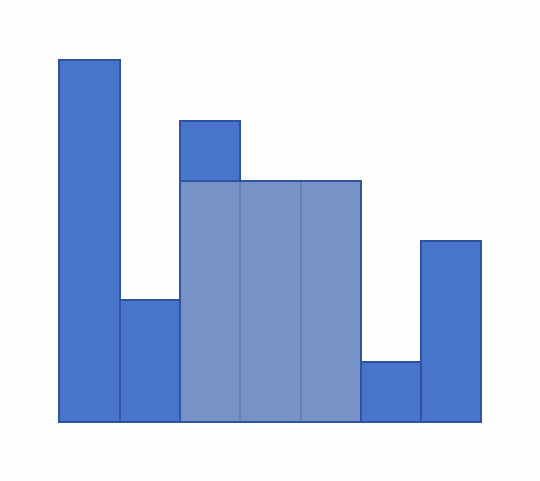
\includegraphics[width=6cm]{withrect.png}
        \caption{The Largest Rectangle in Histogram}
    \end{minipage}
\end{figure}

You may use $Rect(l, r, A)$ to represent the answer of the sub-problem w.r.t. the range $\left[l, r\right]$.

\begin{parts}
    \part[3] \textbf{Briefly} describe:
    \begin{enumerate}
        \item How would you divide the original problem into 2 sub-problems?
        \item Under what circumstances will the answer to the original problem not be covered by the answers of the 2 sub-problems?
        \item Given the answers of the 2 sub-problems, how would you get the answer of the original problem?
    \end{enumerate}
    
    \begin{solution}
    %%%%%%%%%%%%%%%%%%%%%%%%%%%%%%%%%%%%%%%%%%%%%%%%%
    % Replace `\vspace{2in}' with your answer.
    \vspace{2in}
    %%%%%%%%%%%%%%%%%%%%%%%%%%%%%%%%%%%%%%%%%%%%%%%%%
    \end{solution}

    \newpage
    
    \part[8] Based on your idea in part(a), design a \textbf{divide-and-conquer} algorithm for this problem. Make sure to provide \textbf{clear description} of your algorithm design in \textbf{natural language}, with \textbf{pseudocode} if necessary.
    
    \begin{solution}
    %%%%%%%%%%%%%%%%%%%%%%%%%%%%%%%%%%%%%%%%%%%%%%%%%
    % Replace `\vspace{7.5in}' with your answer.
    \vspace{7.5in}
    %%%%%%%%%%%%%%%%%%%%%%%%%%%%%%%%%%%%%%%%%%%%%%%%%
    \end{solution}

    \newpage
    
    \part[2] Provide the run-time complexity analysis of your algorithm in part (b). Make sure to include the \textbf{recurrence relation} of the run-time in your solution.
    
    \begin{solution}
    %%%%%%%%%%%%%%%%%%%%%%%%%%%%%%%%%%%%%%%%%%%%%%%%%
    % Replace `\vspace{3in}' with your answer.
    \vspace{3in}
    %%%%%%%%%%%%%%%%%%%%%%%%%%%%%%%%%%%%%%%%%%%%%%%%%
    \end{solution}
    
\end{parts}